%
% Schnittkrümmung
%
\section{Schnittkrümmung
\label{buch:kruemmung:section:schnittkruemmung}}
\kopfrechts{Schnittkrümmung}
In Beispiel~\ref{buch:kruemmung:kruemmung:bsp:kugel} wurde der 
riemannsche Krümmungstensor einer Kugeloberfläche berechnet.
Es wurde gefunden, dass $R_{1212}=\sin^2\vartheta$ immer noch von der 
Position auf der Kugeloberfläche abhängt.
Wir erwarten aber auch eine Abhängigkeit der Krümmung von der umlaufenen
Fläche.
Der Flächeninhalt eines infinitesimalen Rechtecks mit Seitenlänge
$d\vartheta$ und $d\varphi$ ist
\[
F
=
\sin\vartheta\, d\vartheta\,d\varphi.
\]
Die kovariante riemannsche Tensorkomponenten $R_{1212}$ hängt zweimal
(einmal für jedes Indexpaar $12$) von diesem Flächeninhalt ab.
Wir erwarten daher, dass
\[
K
=
\frac{R_{1212}}{\sin^2\vartheta}
=
1
\]
eine geometrische Invariante ist, die nicht von der Wahl des
Koordinatensystems abhängt.
Dies ist ein Beispiel der Schnittkrümmung, die in diesem Abschnitt
eingeführt werden soll.
Im Gegensatz zu den Komponenten des riemannschen Krümmungstensors ist
die Schnittkrümmung eine geometrische Invariante.
Einerseits lässt sie sich direkt aus dem riemannschen Krümmungstensor
ablesen, der riemannsche Krümmungstensor lässt sich aber auch aus
den Schnittkrümmungen wiedergewinnen.

%
% Geodätische Untermannigfaltigkeiten
%
\subsection{Geodätische Untermannigfaltigkeiten
\label{buch:kruemmung:schnittkrüemmung:subsection:geodum}}
In Abschnitt~\ref{buch:kruemmung:section:flaeche} wurde der
riemannsche Krümmungstensor für eine zweidimensionale riemannsche
Mannigfaltigkeit berechnet.
Es zeigte sich, dass die Information in einer einzigen Zahl,
der gaussschen Krümmung, zusammengefasst werden kann.
In jedem Punkt $p$ einer $n$-dimensionalen Mannigfaltigkeit können für
jedes linear unbhängige Paar von Tangentialvektoren $\vec{h}$ und $\vec{k}$
beliebig viele 2-dimensionale Untermannigfaltigkeiten gefunden werden,
deren Tangentialraum im Punkt $p$ von $\vec{h}$ und $\vec{k}$ aufgespannt
wird.
Die 2-dimensionale Untermannigfaltigkeit hat einen sehr einfachen
Krümmungstensor.
Kann man daraus Information über die ganze Mannigfaltigkeit gewinnen?

Ganz so einfach ist es offenbar nicht, denn der völlig ungekrümmte
3-dimensionale euklidische Raum enthält zum Beispiel Ebenen als
zweidimensionale Untermannigfaltigkeiten, die ebenfalls flach sind,
Kugeloberflächen, die positive Gauss-Krümmung haben, und
Sattelflächen, die negative gausssche Krümmung haben.
Der Unterschied ist jedoch, dass die Geödäten in einer Ebene auch
Geodäten des $\mathbb{R}^3$ sind, während die Geodäten einer 
Kugel $S^2\subset\mathbb{R}^3$ keine Geodäten des $\mathbb{R}^3$
sind.

Wenn eine Fläche in einer $n$-dimensionalen Mannigfaltigkeit aus
Kurven besteht, die stärker gekrümmt sind als die Geodäten 
der $n$-Mannigfaltigkeit, wird es unmöglich, die ``Eigenkrümmung''
dieser Kurven von der Krümmung der umgebenden Mannigfaltigkeit
zu trennen.
Es müssen also 2-dimensionale Mannigfaltigkeiten verwendet werden, 
die aus Geodäten bestehen, die im Punkt $p$ beginnen und als
Tangentialvektor in $p$ eine Linearkombination von $\vec{h}$ und
$\vec{k}$ haben.

%
% Definitin der Schnittkrümmung
%
\subsection{Definition der Schnittkrümmung}
Der riemannsche Krümmungstensor liefert zu einem Bivektor
$\vec{h}\wedge\vec{k}$ eine lineare Abbildung, die die Drehung
eines paralleltransportierten Vektors beschreibt.
Die Abhängigkeit $\vec{h}\wedge\vec{k}\mapsto R(\vec{h}\wedge\vec{k})$
ist bilinear in $\vec{h}$ und $\vec{k}$.
Die Bivektoren aufgespannt von Tangentialvektoren in der
$\vec{h}$-$\vec{k}$-Ebene bilden den eindimensionalen Vektorraum
$\mathbb{R}\vec{h}\wedge\vec{k}$ mit der Basis $\vec{h}\wedge\vec{k}$.

Aus der Theorie der geodätischen Untermannigfaltigkeiten von
Abschnitt~\ref{buch:kruemmung:schnittkrüemmung:subsection:geodum}
ergibt sich, dass Tangentialvektoren in der $\vec{h}$-$\vec{k}$-Ebene
in dieser Ebene bleiben.
Der Wert $R(\vec{h}\wedge\vec{k})$ beschreibt eine infinitesimale Drehung
in der $\vec{h}\wedge\vec{k}$-Ebene.
In einer orthonormierten Basis wird sie beschrieben durch eine
antisymmetrische Matrix.
Die Antisymmetrie bedeutet, dass der Wert $R(\vec{h}\wedge\vec{k})$ ist
also wieder ein Vielfaches von $\vec{h}\wedge\vec{k}$, es gibt
eine Zahl $s(\vec{h}\wedge\vec{h})$ mit der Eigenschaft
\[
R(\vec{h}\wedge\vec{k})
=
s(\vec{h}\wedge\vec{k})
\vec{h}\wedge\vec{k}.
\]
Da $R(\vec{h}\wedge\vec{k})$ linear von $\vec{h}\wedge\vec{k}$ abhängt,
muss auch $s(\vec{h}\wedge\vec{k})$ linear von $\vec{h}\wedge\vec{k}$
abhängen.

Der Bivektor $\vec{h}\wedge\vec{k}$ repräsentiert den Flächeninhalt
des von $\vec{h}$ und $\vec{k}$ aufgespannten Parallelogramms. 
In einer orthonormierten Basis wird es durch die Determinante wiedergegeben,
die mit $|\vec{h}\wedge\vec{k}|$ geschrieben werden kann.
es muss also ein Zahl $S$ geben derart, dass
\[
R(\vec{h}\wedge\vec{k})
=
s(\vec{h}\wedge\vec{k})
\begin{pmatrix*}[r] 0&-1\\ 1&0\end{pmatrix*}
|\vec{h}\wedge\vec{k}|
=
S |\vec{h}\wedge\vec{k}|^2
\begin{pmatrix*}[r] 0&-1\\1&0\end{pmatrix*}.
\]
Der Faktor $S$ ist unabängig von der Basis in der $\vec{h}$-$\vec{k}$-Ebene
und damit eine innere Eigenschaft der Mannigfaltigkeit.

\begin{definition}[Schnittkrümmung]
\label{buch:kruemmung:schnittkruemmung:def:schnittkruemmung}
Sie $M$ eine riemannsche Mannigfaltigkeit mit dem kovarianten riemannschen
Krümmungstensor $Rm(X,Y,Z,W)$.
Die Grösse
\[
S(X\wedge Y) = \frac{Rm(X,Y,X,Y)}{|X\wedge Y|^2}.
\]
heisst die \emph{Schnittkrümmung} in der von $X$ und $Y$ aufgespannten
geodätischen Untermannigfaltigkeit von $M$.
\index{Schnittkrümmung}%
\end{definition}

\begin{beispiel}
Wir betrauchten den Graphen einer Funktion $z=f(x,y)$.
Die Metrik wird 
durch die Gram-Matrix der Einbettung
\[
\vec{r}
\colon
\mathbb{R}^2 \to \mathbb{R}^3
:
(u,v)
\mapsto 
\begin{pmatrix} u \\ v \\ f(u,v) \end{pmatrix}
\]
beschrieben und wurde bereits in
Beispiel~\ref{buch:kruemmung:flaeche:bsp:gram}
als
\[
g
=
\begin{pmatrix}
1 + f_u(u,v)^2    & f_u(u,v) f_v(u,v) \\
f_u(u,v) f_v(u,v) & 1 + f_u(u,v)^2
\end{pmatrix}
\]
berechnet.
Daraus kann man mit einer ziemlich aufwendigen Rechnung, die man
mit Vorteil von einem Computeralgebrasystem durchführen lässt
(Maxima-Script \texttt{f.maxima} im Source-Code-Repository des Buches)
den riemannschen Krümmungstensor berechnen kann.

Um den Ausdruck besser zu verstehen beschränken wir uns auf eine Stelle,
wo $f_u(u,v)=f_v(u,v)=0$ gilt.
Die Rechnung liefert dann
\[
R_{1212} = f_{uu}(u,v) f_{vv}(u,v) - f_{uv}(u,v)^2.
\]
Für die Schnittkrümmung muss der Flächeninhalt des von den Tangentialvektoren
\[
\partial_u
=
\partial/\partial u
=
\begin{pmatrix}1\\0\\0\end{pmatrix}
\qquad\text{und}\qquad
\partial_v
=
\partial/\partial v
=
\begin{pmatrix}0\\1\\0\end{pmatrix}
\]
aufgespannten Parallelogramms berechnet werden.
Die beiden Vektoren sind orthogonale Einheitsvektoren, also ist
der Flächinhalt $|\partial_u\wedge\partial_v|=1$ und damit ist
\[
S
=
f_{uu}(u,v) f_{vv}(u,v) - f_{uv}(u,v)^2
\]
die Schnittkrümmung.
Sie stimmt überein mit der früher gefundenen gaussschen Krümmung
der Fläche.
\end{beispiel}

%
% Abstand von Geodäten
%
\subsection{Abstand von Geodäten}
%
% fig-abstandtex
%
% (c) 2025 Prof Dr Andreas Müller
%
\begin{figure}
\centering
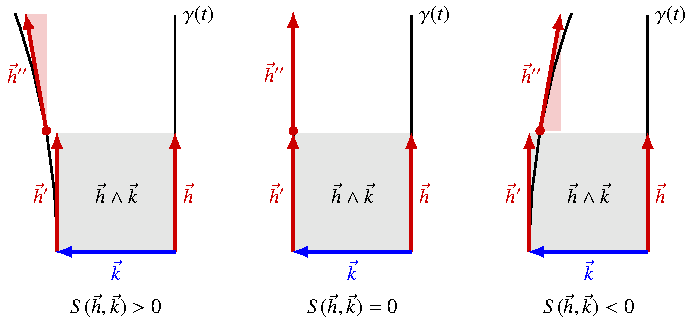
\includegraphics{chapters/110-kruemmung/images/abstand.pdf}
\caption{Schnittkrümmung und der Abstand von Geodäten mit
parallelverschobener Anfangsrichtung, die von infinitesimal
benachbarten Punkten ausgehen.
Bei positiver Schnittkrümmung wird der Abstand grösser, bei negtiver
Schnittkrümmung wird er kleiner.
\label{buch:kruemmung:schnittkruemmung:fig:abstand}}
\end{figure}

Die Schnittkrümmung codiert auch, sich der Abstand von Geodäten,
die in geringem Abstand aber mit paralleltransportierter Richtung
beginnen.
Dazu betrachten wir eine Geodäte mit Tangente $\vec{h}$ und
vergleichen Sie mit einer Geodäte, deren Anfangspunkt infinitesimal
in Richtung $\vec{k}$ verschoben ist.

Ist die Schnittkrümmung $S(\vec{h},\vec{k})=0$, dann dreht sich der
Tangentialvektor beim Paralleltransport nicht.
In der Abbildung~\ref{buch:kruemmung:schnittkruemmung:fig:abstand}
in der Mitte wird dies dadurch angezeigt, dass der Vektor $\vec{h}''$
seine Richtung nicht geändert hat.

Bei positiver Schnittkrümmung, dargestellt in
Abbildung~\ref{buch:kruemmung:schnittkruemmung:fig:abstand}
links, dreht sich der Tangentialvektor in positiver Richtung und der
Abstand zwischen den Geodäten wird grösser.
Umgekehrt dreht sich bei negativer Schnittkrümmung, dargestellt in
Abbildung~\ref{buch:kruemmung:schnittkruemmung:fig:abstand} rechts,
der Tangentialvektor $\vec{h}''$ im Uhrzeigersinn, der Abstand
der Geodäten wird kleiner.

Man kann die Abstandsänderung auch direkt aus den Rechenregeln für
die kovariante Ableitung berechnen, für unsere Zwecke soll die
intuitive graphische Erklärung von 
Abbildung~\ref{buch:kruemmung:schnittkruemmung:fig:abstand}
genügen.

Später in Abschnitt~\ref{buch:kruemmung:section:newton} wird gezeigt,
dass die Abstandsänderung als gravitative Wirkung interpretiert
werden kann.
Damit ist bereits angedeutet, was die allgemeine Relativitätstheorie
beweist, dass nämlich Gravitation durch die Krümmung der Raum-Zeit
beschrieben werden kann.

%
% Schnittkrümmungen bestimmen den riemannschen Krümmungstensor
%
\subsection{Schnittkrümmungen bestimmen den riemannschen
Krüm\-mungs\-ten\-sor}

\begin{satz}
Der riemannsche Krümmungstensor einer Mannigfaltigkeit $M$
ist vollständig bestimmt durch die Schnittkrümmungen.
\end{satz}

Der Beweis wird zeigen, dass sich sogar eine konkrete Formel
für die Werte des Krümmungstensors angeben lässt.

\begin{proof}
Die Komponenten $R_{lhik}$ des riemannsche Krümmungstensors ist
antisymmetrisch im ersten und letzten Indexpaar.
Es gilt also
\[
R_{lhik}
-R_{hlik}
=
-R_{lhki}.
\]
Dies bedeutet, dass die 4-Linearform
\[
Rm(X,Y,Z,W)
=
\xi^l\eta^h\zeta^i\omega^k R_{lhik}
\]
nur von den 2-Vektoren $X\wedge Y$ bzw.~$Z\wedge W$ abhängt.
Der Krümmungstensor kann daher auch als blineare Funktion
\begin{equation}
\bigwedge^2 TM\otimes\bigwedge^2 TM
\to
\mathbb{R}
:
(X\wedge Y,Z\wedge W)
\mapsto
R(X\wedge Y, Z\wedge W)
=
Rm(X,Y,Z,W)
\label{buch:kruemmung:schnittkruemmung:eqn:Rbivektor}
\end{equation}
auf dem Vektorraum $\bigwedge^2 TM$ der 2-Vektoren von Tangentialvektoren
geschrieben werden.

Der Krümmungstensor ist ausserdem symmetrisch unter der Vertauschung
der Indexpaare $lh$ und $ik$.
Dies bedeutet, dass die
in
\eqref{buch:kruemmung:schnittkruemmung:eqn:Rbivektor}
definierte Funktion $R$ auf den 2-Vektoren symmetrisch ist:
\begin{align*}
R(X\wedge Y,Z\wedge W)
=
R(Z\wedge W,X\wedge Y)
\end{align*}
für beliebige 2-Vektoren $X\wedge Y,Z\wedge W\in\bigwedge^2TM$.
Wir schreiben die symmetrische, bilineare Funktion auch als $R(u,v)$ mit
$u,v\in\bigwedge^2 TM$.

Wir möchten zeigen, dass sich $R(u,v)$ aus den Werten $R(w,w)$ für beliebige
2-Vektoren $w$ berechnen lässt.
Um dies etwas prägnanter auszudrücken, schreiben wir
\[
Q(w) = R(w,w).
\]
Die Funktion $Q$ ist eine quadratische Form.

Die Polarisationsformel \cite[p. 347]{buch:linalg} besagt, dass eine
symmetrische, bilineare Funktion $R(u,v)$ vollständig durch die
Werte $R(u,v)$ bestimmt ist.
Wir führen die Rechnung 
\begin{align}
R(u+v,u+v)
&=
R(u,u) + R(u,v) + R(v,u) + R(v,v)
\notag
\\
\Rightarrow\qquad
Q(u+v)
&=
R(u,u) + 2R(u,v) + R(v,v)
\notag
\\
R(u-v,u-v)
&=
R(u,u) - R(u,v) - R(v,u) + R(v,v)
\notag
\\
\Rightarrow\qquad
Q(u-v)
&=
R(u,u) - 2R(u,v) + R(v,v)
\notag
\intertext{mit der Differenz}
Q(u+v)-Q(u-v)
&=
4 R(u,v),
\notag
\intertext{oder aufgelöst nach dem gemischten Term:}
R(u,v)
&=
{\textstyle\frac14}\bigl( Q(u+v) - Q(u-v) \bigr).
\label{buch:kruemmung:schnittkruemmung:eqn:RQQ}
\end{align}
Die Formel \eqref{buch:kruemmung:schnittkruemmung:eqn:RQQ}
drückt $R(u,v)$ durch Werte der Form $R(w,w)$ mit $w\in\bigwedge^2 TM$ aus.
\end{proof}

\begin{satz}
Der Krümmungstensor ist durch die Schnittkrümmungen vollständig
bestimmt.
\end{satz}

\begin{proof}
Die Schnittkrümmung zu den Vektoren $\vec{s}$ und $\vec{v}$ ist
definiert durch
\begin{align}
K(\vec{s},\vec{v})
&=
\frac{
R(\vec{v},\vec{s},\vec{v},\vec{s})
}{
|\vec{v}\wedge\vec{s}|^2
}.
\intertext{Für einen Basis-2-Vektor $\vec{e}_i\wedge\vec{e}_k$ wird dies zu}
K(\vec{e}_i,\vec{e}_k)
&=
\frac{Rm(\vec{e}_i,\vec{e}_k,\vec{e}_i,\vec{e}_k)}{|\vec{e}_i\wedge\vec{e}_k|^2}
\notag
\\
&=
\frac{R_{ikik}}{g^{ii}g^{kk}-g^{ik}g^{ik}}.
\label{buch:kruemmung:schnittkruemmung:eqn:Rgggg}
\end{align}
Da $g$ als Metrik definit ist, ist der Nenner von
\eqref{buch:kruemmung:schnittkruemmung:eqn:Rgggg}
niemals 0.
Der Riemannsche Krümmungstensor kann also aus den Werten
\[
Rm(\vec{e}_i,\vec{e}_k,\vec{e}_i,\vec{e}_k)
=
R(\vec{e}_i\wedge\vec{e}_k,\vec{e}_i\wedge\vec{e}_k)
=
Q(\vec{e}_i\wedge\vec{e}_k)
=
(g^{ii}g^{kk}-g^{ik}g^{ik}) K(\vec{e}_i,\vec{e}_k)
\]
bestimmt werden.
Sie können also aus den Schnittkrümmungen ermittelt werden.
\end{proof}

Der Satz besagt also, dass die vom riemannschen Krümmungstensor
beschriebene Krümmung des Raumes vollständig ergründet werden kann,
indem man Messungen in divergierenden Gedäten durchführt.
Eine andere Art, dies auszudrücken, ist, dass der riemannsche
Krümmungstensor keine zusätzliche Information erhält, die man nicht
in der Funktion der Schnittkrümmungen gefunden werden kann.

